\documentclass{beamer}
\usepackage{tfrupee} 
\usepackage[utf8]{inputenc}
\usepackage{lmodern} 
\usepackage[utf8]{inputenc}
\usepackage{lmodern} 
\usepackage{listings}
\usepackage{xcolor} 
\usepackage{graphicx}
\definecolor{myblue}{RGB}{48, 63, 159}
\setbeamercolor{palette primary}{bg=myblue, fg=white}
\setbeamercolor{structure}{fg=myblue}
\setbeamercolor{frametitle}{bg=myblue, fg=white}
\setbeamercolor{title}{bg=myblue, fg=white}
\setbeamercolor{footlinecolor}{bg=myblue, fg=white}


\defbeamertemplate*{title page}{mytemplate}{
	\vfill
	\begin{center}
		
		\begin{beamercolorbox}[wd=0.8\paperwidth, center, rounded=true, shadow=true]{title}
			\usebeamerfont{title}\inserttitle\par
		\end{beamercolorbox}
		\vspace{2cm} 
		
		\usebeamerfont{author}\insertauthor
		\vspace{1cm} 
		\usebeamerfont{date}\insertdate
	\end{center}
	\vfill
}


\defbeamertemplate*{frametitle}{mytemplate}{
	\begin{beamercolorbox}[wd=\paperwidth, ht=2.5ex, dp=1.5ex, left]{frametitle}
		\hspace{1em}\usebeamerfont{frametitle}\insertframetitle
	\end{beamercolorbox}
}


\setbeamertemplate{footline}{
	\begin{beamercolorbox}[wd=\paperwidth, ht=2.25ex, dp=1ex]{footlinecolor}
		\hspace{1em}\usebeamerfont{author in footline}\insertshortauthor
		\hfill
		\usebeamerfont{title in footline}\insertshorttitle
		\hfill
		\usebeamerfont{date in footline}\insertdate \hspace{1em} \insertframenumber/\inserttotalframenumber \hspace{0.5em}
	\end{beamercolorbox}
}


\setbeamerfont{author in footline}{size=\tiny}
\setbeamerfont{title in footline}{size=\tiny}
\setbeamerfont{date in footline}{size=\tiny}

\newcommand{\myvec}[1]{\ensuremath{\begin{pmatrix}#1\end{pmatrix}}}
\providecommand{\brak}[1]{\ensuremath{\left(#1\right)}}


\title{5.9.7}
\author{Shriyansh Chawda-EE25BTECH11052}




\begin{document}
	

		\setbeamertemplate{footline}{} 
		\frame{\titlepage}
	
	
\begin{frame}{Question} 
	A part of monthly hostel charges in a college hostel are fixed and the remaining depends on the number of days one has taken food in the mess. When a student A takes food for 25 days, he has to pay \rupee 4,500, whereas a student B who takes food for 30 days, has to pay \rupee 5,200. Find the fixed charges per month and the cost of
food per day.
\hfill{(10, 2019)}
\end{frame}
	
\begin{frame}{Solution}
Let x be the fixed charge and y be the cost of food per day.\\
The system according to the information is
\begin{align}
	x + 25y &= 4500 \\
	x + 30y &= 5200
\end{align}
In matrix form:
\begin{align}
	\myvec{1 & 25 \\ 1 & 30} \myvec{x \\ y} = \myvec{4500 \\ 5200}.
\end{align}
Let
\begin{align}
	A = \myvec{1 & 25 \\ 1 & 30}, \quad \vec{b} = \myvec{4500 \\ 5200}.
\end{align}
Solving it using Gauss-Jordan elimination, we get
\end{frame}



\begin{frame}{Solution}
\begin{align}
	\left[\begin{array}{cc|c}
		1 & 25 & 4500 \\
		1 & 30 & 5200
	\end{array}\right]
	&\xrightarrow{R_2 \rightarrow R_2 - R_1}
	\left[\begin{array}{cc|c}
		1 & 25 & 4500 \\
		0 & 5 & 700
	\end{array}\right] \\
	&\xrightarrow{R_2 \rightarrow \tfrac{1}{5}R_2}
	\left[\begin{array}{cc|c}
		1 & 25 & 4500 \\
		0 & 1 & 140
	\end{array}\right] \\
	&\xrightarrow{R_1 \rightarrow R_1 - 25R_2}
	\left[\begin{array}{cc|c}
		1 & 0 & 1000 \\
		0 & 1 & 140
	\end{array}\right]
\end{align}
From the reduced row echelon form, we have the solution:
\begin{align}
	\myvec{x \\ y} = \myvec{1000 \\ 140}
\end{align}
Therefore,
\begin{align}
	x = 1000 \quad \text{(fixed charge)}, \qquad y = 140 \quad \text{(cost per day)}.
\end{align}
\end{frame}
\begin{frame}{Plot}
\begin{figure}[H]
	\centering
	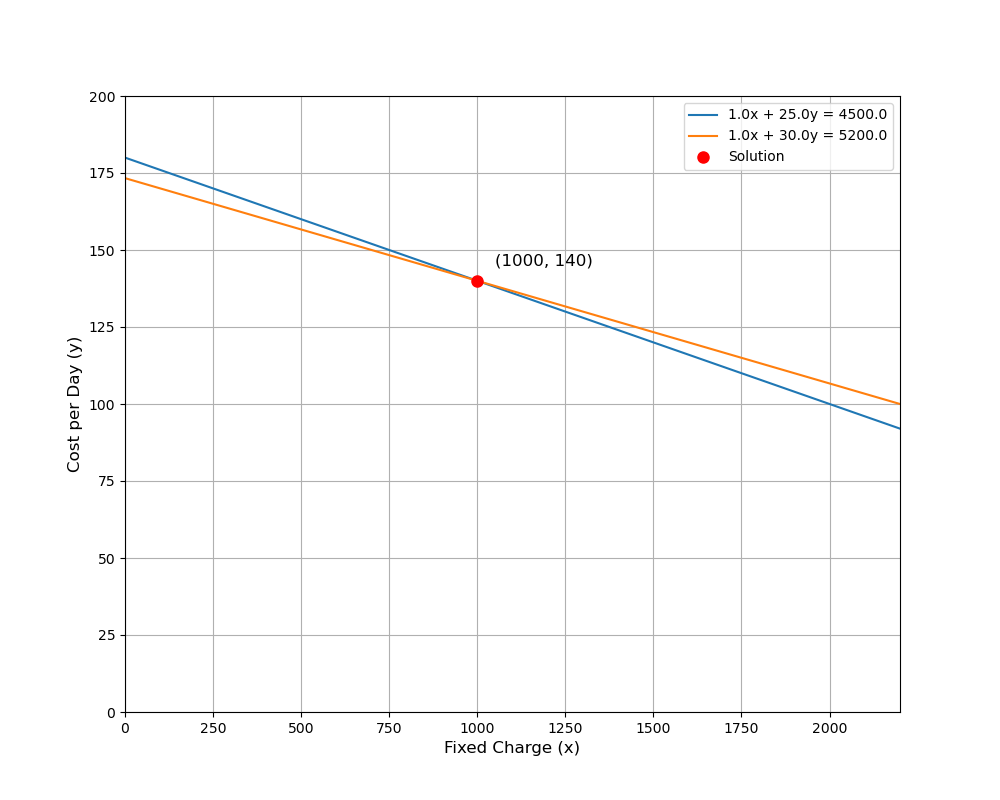
\includegraphics[width=0.9\linewidth]{figs/hostel_charges_plot}
\end{figure}

\end{frame}
 



\end{document}